%
% fig-nullstellen.tex
%
% (c) 2026 Prof Dr Andreas Müller
%
\begin{figure}
	\centering
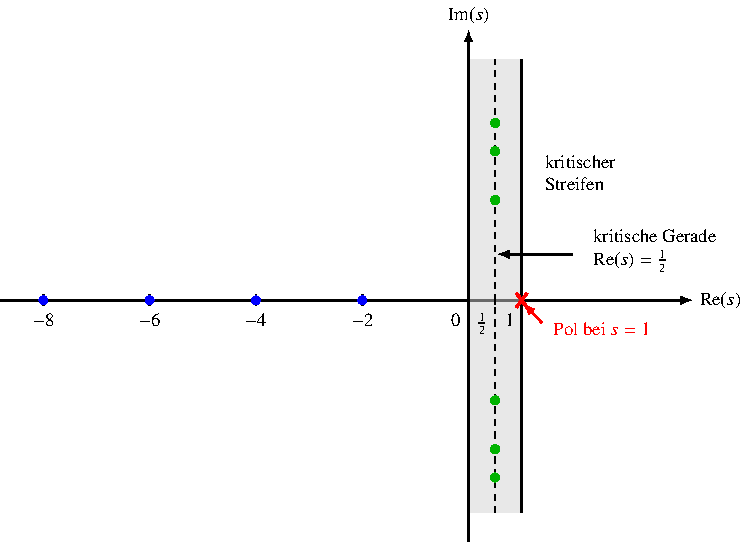
\includegraphics{papers/hankel/images/nullstellen.pdf}
%	
%	\begin{tikzpicture}[x=0.9cm,y=0.12cm,font=\small,>=latex]
%		
%		% ------------------------------------------------------------
%		% Achsen
%		% ------------------------------------------------------------
%		\draw[->] (-8.8,0) -- (4.2,0) node[right] {$\Re(s)$};
%		\draw[->] (0,-34) -- (0,38) node[above] {$\Im(s)$};
%		
%		% ------------------------------------------------------------
%		% Kritischer Streifen 0 < Re(s) < 1
%		% ------------------------------------------------------------
%		\fill[gray!18] (0,-30) rectangle (1,34);
%		\draw[thick] (0,-30) -- (0,34);
%		\draw[thick] (1,-30) -- (1,34);
%		
%		% kritische Gerade Re(s)=1/2
%		\draw[dashed,thick] (0.5,-30) -- (0.5,34);
%		
%		% ------------------------------------------------------------
%		% Markierungen auf der reellen Achse
%		% ------------------------------------------------------------
%		\foreach \x in {-8,-6,-4,-2,0,1}
%		{
%			\draw (\x,0.8) -- (\x,-0.8);
%		}
%		
%		\draw (0.5,0.6) -- (0.5,-0.6);
%		
%		\node[below] at (-8,-0.8) {$-8$};
%		\node[below] at (-6,-0.8) {$-6$};
%		\node[below] at (-4,-0.8) {$-4$};
%		\node[below] at (-2,-0.8) {$-2$};
%		
%		\node[below left]  at (0,-0.8) {$0$};
%		\node[below left]       at (0.5,-0.6) {$\frac12$};
%		\node[below left] at (1,-0.8) {$1$};
%		
%		% ------------------------------------------------------------
%		% triviale Nullstellen
%		% ------------------------------------------------------------
%		\foreach \x in {-8,-6,-4,-2}
%		{
%			\fill[blue] (\x,0) circle (2.1pt);
%		}
%		
%		%\node[align=center] at (-6.1,-12)
%		%{
%		%	triviale\\
%		%	Nullstellen
%		%};
%		
%		%\draw[->,green] (-5.95,-9.2) -- (-2.02,-0.5);
%		%\draw[->,green] (-5.95,-9.2) -- (-4.02,-0.5);
%		%\draw[->,green] (-5.95,-9.2) -- (-6.02,-0.5);
%		%\draw[->,green] (-5.95,-9.2) -- (-8.02,-0.5);
%		% ------------------------------------------------------------
%		% nichttriviale Nullstellen
%		% echte erste paar Ordinaten, alle auf Re(s)=1/2
%		% ------------------------------------------------------------
%		\foreach \y in {14.1347,21.0220,25.0109,-14.1347,-21.0220,-25.0109}
%		{
%			\fill[green!70!black] (0.5,\y) circle (2.2pt);
%		}
%		
%		% ------------------------------------------------------------
%		% Beschriftung kritischer Streifen
%		% ------------------------------------------------------------
%		\node[align=left] at (2.1,18)
%		{
%			kritischer\\
%			Streifen
%		};
%		
%		% kritische Gerade
%		\node[align=left] at (3.5,7)
%		{
%			kritische Gerade\\
%			$\Re(s)=\frac12$
%		};
%		
%		\draw[->] (1.95,6.5) -- (0.56,6.5);
%		
%		% nichttriviale Nullstellen
%		%\node[align=right] at (-1.5,23)
%		%{
%		%	nichttriviale\\
%		%	Nullstellen
%		%};
%		
%		%\draw[->,blue] (-0.55,21.5) -- (0.44,-14.1);
%		%\draw[->,blue] (-0.55,21.5) -- (0.44,-21.0);
%		%\draw[->,blue] (-0.55,21.5) -- (0.44,-25.0);
%		%\draw[->,blue] (-0.55,21.5) -- (0.44,25.0);
%		%\draw[->,blue] (-0.55,21.5) -- (0.44,21.0);
%		%\draw[->,blue] (-0.55,21.5) -- (0.44,14.1);
%		% ------------------------------------------------------------
%		% Pol bei s=1
%		% ------------------------------------------------------------
%		\draw[red,very thick] (0.90,-1.0) -- (1.10,1.0);
%		\draw[red,very thick] (0.90,1.0) -- (1.10,-1.0);
%		
%		\node[red,anchor=west] at (1.45,-4.0) {Pol bei $s=1$};
%		\draw[->,red] (1.38,-3.2) -- (1.05,-0.5);
%		
%	\end{tikzpicture}
	
	\caption{
		Darstellung der Nullstellen der Riemannschen Zetafunktion.
		Die \textcolor{blue}{trivialen Nullstellen} liegen bei den negativen geraden Zahlen.
		Der graue Bereich bezeichnet den kritischen Streifen \(0<\Re(s)<1\),
		die gestrichelte Linie die kritische Gerade \(\Re(s)=\tfrac12\).
		Die eingezeichneten ersten \textcolor{green!70!black}{nichttrivialen Nullstellen} liegen bei
		\(\tfrac12 \pm 14.1347\,i\),
		\(\tfrac12 \pm 21.0220\,i\) und
		\(\tfrac12 \pm 25.0109\,i\).
		Ausserdem besitzt \(\zeta(s)\) bei \(s=1\) einen einfachen Pol.
	}
	\label{hankel:fig:nullstellen}
\end{figure}
